\documentclass{standalone}
\usepackage{pgfplots}
\usepackage{pgfplotstable}
\pgfplotsset{compat=1.16}
\usetikzlibrary{matrix,chains,trees,scopes,decorations,arrows.meta,automata,positioning,shadows,3d}




\begin{document}
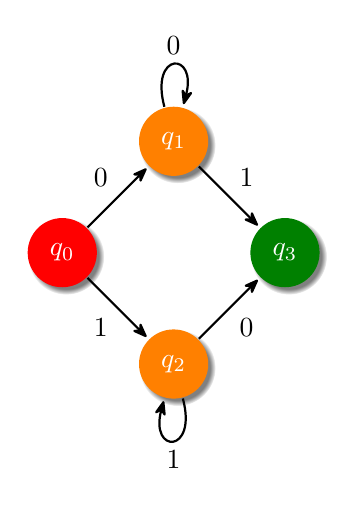
\begin{tikzpicture}[shorten >=1pt,node distance=2cm,on grid,>={Stealth[round]},thick,
    every state/.style={fill,draw=none,orange,text=white,circular drop shadow},
    accepting/.style ={green!50!black,text=white},
    initial/.style ={red,text=white}]
    \node[state,initial] (q_0) {$q_0$};
    \node[state] (q_1) [above right=of q_0] {$q_1$};
    \node[state] (q_2) [below right=of q_0] {$q_2$};
    \node[state,accepting](q_3) [below right=of q_1] {$q_3$};
    \path[->] (q_0) edge node [above left] {0} (q_1)
    edge node [below left] {1} (q_2)
    (q_1) edge node [above right] {1} (q_3)
    edge [loop above] node {0} ()
    (q_2) edge node [below right] {0} (q_3)
    edge [loop below] node {1} ();
\end{tikzpicture}
\hspace*{8em}
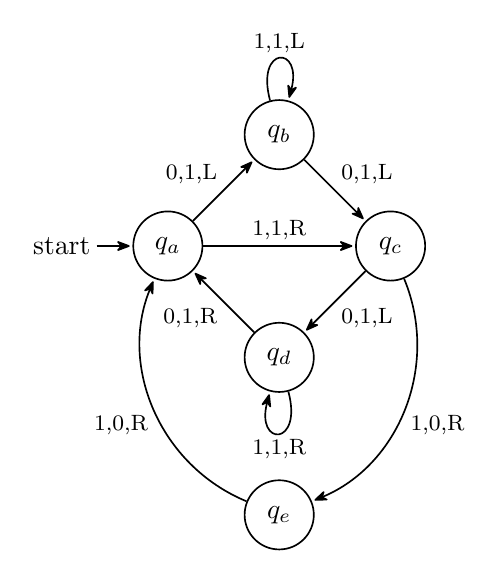
\begin{tikzpicture}[->,>={Stealth[round]},shorten >=1pt,%
    auto,node distance=2cm,on grid,semithick,
    inner sep=2pt,bend angle=45]
    \node[initial,state] (A) {$q_a$};
    \node[state] (B) [above right=of A] {$q_b$};
    \node[state] (D) [below right=of A] {$q_d$};
    \node[state] (C) [below right=of B] {$q_c$};
    \node[state] (E) [below=of D] {$q_e$};
    \path [every node/.style={font=\footnotesize}]
    (A) edge node {0,1,L} (B)
    edge node {1,1,R} (C)
    (B) edge [loop above] node {1,1,L} (B)
    edge node {0,1,L} (C)
    (C) edge node {0,1,L} (D)
    edge [bend left] node {1,0,R} (E)
    (D) edge [loop below] node {1,1,R} (D)
    edge node {0,1,R} (A)
    (E) edge [bend left] node {1,0,R} (A);
\end{tikzpicture}
\end{document}